\documentclass{llncs}
\usepackage{times, epsfig,booktabs}
\usepackage{amsmath,amssymb}

\usepackage[linesnumbered,ruled,vlined]{algorithm2e} 
\usepackage{multicol}

\usepackage{fancyvrb}
\usepackage{comment}
\usepackage{graphicx} 
\usepackage{subfigure}

\usepackage{paralist} 
\usepackage{multirow}
\usepackage{array} 
\usepackage{slashbox}

\usepackage{endnotes}
\usepackage{footnote}


\begin{document}
\setlength{\intextsep}{2pt}
\setlength{\textfloatsep}{2pt}

\title{Identifying Hesitant and Interested Customers for Targeted Social Marketing}

\author{Guowei Ma \and Qi Liu \and Le Wu  \and Enhong Chen }
\institute{University of Science and Technology of China\\
\email{\{gwma,wule\}@mail.ustc.edu.cn}, \email{\{qiliuql,cheneh\}@ustc.edu.cn}
}

\maketitle
\begin{abstract}
Social networks provide unparalleled opportunities for marketing products or services. Along this line, tremendous efforts have been devoted to the research of targeted social marketing, where the marketing efforts could be concentrated on a particular set of users with high utilities.
Traditionally, these targeted users are identified based on their potential interests to the given company (product). However, social users are usually influenced simultaneously by multiple companies, and not only the user interest but also these social influences will contribute to the user consumption behaviors. To that end, in this paper, we propose a general approach to figure out the targeted users for social marketing, taking both user interests and multiple social influences into consideration. Specifically, we first formulate it as an Identifying Hesitant and Interested Customers (IHIC) problem, where we argue that these valuable users should have the best balanced influence entropy (being ``Hesitant'') and utility scores (being ``Interested''). Then, we design a novel framework and propose specific algorithms to solve this problem. Finally, extensive experiments on two real-world datasets validate the effectiveness and the efficiency of our proposed approach.
\end{abstract}


\vspace*{-0.3cm}
\section{Introduction} \label{sec:intro}
\vspace*{-0.3cm}

Recent years have witnessed the development of the social networking services and famous companies usually have their official accounts on many social network sites. For instance, Samsung, Huawei, HTC, and Xiaomi, all have their official accounts on Weibo, (weibo.com, the largest social platform in China). As users on social networks will follow the users (companies) they are interested in and receive messages and information posted by these followees \cite{kwak2010twitter}, social network sites (e.g., Twitter, Facebook and Weibo) have become new resources and platforms to conduct marketing campaign \cite{hartline2008optimal}. 


Like traditional marketing strategies, it is also essential to figure out one or a few customer segments to target on for social marketing \cite{liu2013conducting}. These targeted users should have high utilities, and then the marketing efforts (e.g., personalized recommendation \cite{kantor2011recommender}, viral marketing \cite{kempe2003maximizing}) could be concentrated on them. Generally speaking, both user profiles \cite{alowibdi2013empirical} and user's historical consumption records \cite{jamali2009trustwalker} are helpful for measuring their potential interests to the given company (product). On the other hand, since multiple companies simultaneously have their accounts in the social network, they will significantly
influence social users' choice \cite{he2012influence,chen2013information}. Thus, when conducting targeted social marketing, the given company should consider both user interests and the social influences as they will contribute to the users' final consumption behaviors.

For instance, during one targeted social marketing campaign for Samsung, we find three candidate targeted users $u_1$, $u_2$, $u_3$ may be interested in the products of Samsung (Interested Customers, i.e., mined based on their consumption records). Then, the problem becomes who is the most valuable user among them? Suppose there are two other competing companies of Samsung: Huawei and HTC, and suppose we could compute that the influence value distribution from these three companies to the three users are $[0.8,0.1,0.1]$ for $u_1$, $[0.1,0.1,0.8]$ for $u_2$, $[0.35,0.34,0.31]$ for $u_3$, respectively. Let's take $u_3$ as an example, it means that $u_3$ has the probability of 35\%,34\%,31\% to be influenced by Samsung, Huawei, HTC, respectively. 
If these three users showed the similar interests to Samsung, then the most valuable user for targeted marketing should be $u_3$ rather than $u_1$ and $u_2$. Actually, $u_1$ is already a big fun of Samsung and thus we do not have to market on him, while $u_2$ is deeply influenced by our competitor (i.e., HTC) and thus he will have lower probability to choose our product\footnote{We will support this assumption by experimental analysis.}. Furthermore, it means we should spare our energy for other users, e.g., $u_3$, who has not been deeply influenced by any company and has no bias on any company (we call these users as the ``Hesitant Customers''). If we pay attention on $u_3$, this user may choose our products. Thus, $u_3$ is actually the most valuable user that Samsung should market on. In summary, we argue that when the companies want to market their products, it's energy-efficient for them to target on the users, who not only have the interest to buy the specific product (e.g., one Smartphone) but also have no bias on any company and have not yet decided to choose which company's products (such as Samsung Galaxy or HTC one).


In this paper, we formulate the problem of figuring out these targeted users, like $u_3$, as an Identifying Hesitant and Interested Customers (IHIC) problem. As a matter of fact, there are several challenges along this line, e.g., how to compute the multiple companies' influences on users efficiently,  how to measure the user hesitancy and the user interest. To address these challenges and to solve the IHIC problem effectively and efficiently, we design a novel framework. Specifically, we first propose an efficient algorithm(MIP) to compute the multiple companies' influences  on users, and  identify the hesitant customers by using hesitant functions. Then, we use the collaborative filtering approaches to measure the user's utilities (interests). Finally, the targeted users are those having the best balanced hesitancy scores and utility scores. Extensive experimental results demonstrate that the targeted users selected by our framework could bring in more benefit for the company than the users who are only interested or hesitant.


To the best of our knowledge, this is the first attempt on a comprehensive study of targeted marketing that considers both user interests and multiple social influences. Our solution could identify the most profitable
potential targeted users to optimize the marketing performance. Meanwhile, the
proposed targeted marketing approach is a general framework and each step could be open to some other algorithms. 



%%%%%%%%%%%%%%%%%%%%%%%% Related Work %%%%%%%%%%%%%%%%%%%%%%%%%%%%%%%%%%%%%%
\vspace*{-0.4cm}
\section{Related Work}
\vspace*{-0.4cm}

Marketers incline to conduct marketing campaign on social networks by employing various techniques and approaches~\cite{hartline2008optimal}, and some of them focus on (1) identifying the targeted customers who maybe interested in the specific product, or (2) exploiting the information diffusion effect to influence social customers' consumption decisions.

For identifying targeted customers \cite{tang2013social,koren2009matrix}, the techniques that are related to recommender systems could be easily adopted. Along this line, there are generally three types of techniques: content-based, collaborative filtering and social recommendations. The content-based methods leverage users' profile (e.g., age, job, and location) to predict whether the user's interest matches the product~\cite{contentRS2007}. In contrast, collaborative filtering usually relies on users' past behaviors without requiring the explicit profiles\cite{cf2009survey}. Furthermore, the social recommendation takes the users' social ties into consideration and predicts a user's interest based on his neighbors' interests~\cite{tang2013social}. In real world scenarios, hybrid techniques are also widely used, for instance, Jamali et al. proposed to combine the social-based and the collaborative filtering approaches together to infer customer preference \cite{jamali2009trustwalker}. Unfortunately, few existing studies in this category pay attention to mining the influences coming from the companies to customers.


For exploiting the information diffusion effect, i.e., social influence, researchers first try to learn the information propagation probability between two social neighbors \cite{goyal2010learning,kdd13STRIP}.  Then some related work proposed to model/simulate the entire process of information propagation, e.g., Independent Cascade (IC) model~\cite{goldenberg2001talk} and Linear Threshold (LT) model~\cite{granovetter1978threshold} are two widely used ones. However, both of them require Monto Carlo simulations to estimate the influence spread, which is very time-consuming; some efficient (or tractable) influence models are proposed, such as the stochastic information flow model~\cite{aggarwal2011flow} and the linear social influence (Linear) model~\cite{ijcai13biaoxiang}. Though it's convenient for these models to get the influences of a given node on others, the computation of the influences from multiple seed nodes on a given node is still inefficient. Actually, we will address this inefficiency problem by proposing a novel way of computing the influences from multiple companies on users. Meanwhile, note that social influence is often used to change customers' consumption decisions in viral marketing (e.g., via social influence maximization)~\cite{kempe2003maximizing,chen2013information}, in this paper, we will show that it could also be helpful for targeted social marketing (i.e., identifying targeted customers).



%%%%%%%%%%%%%%%%%%%%% Problem Statement and Formulation %%%%%%%%%%%%%%%%%%%%%%%%%
\vspace*{-0.4cm}
\section{Problem Statement and Formulation}
\vspace*{-0.4cm}

The nodes in social networks could generally be classified into two categories, namely users' personal accounts and companies' official accounts. Usually, each company may maintain several official accounts at the same time. E.g., both ``Xiaomi mobile'' and ``Xiaomi Company'' are all official accounts of the \emph{Xiaomi} Company on Weibo. Here, let the directed graph $G(V,E,T)$ represent a social network, where $V= C\cup U=\{1,2,...,c\}\cup \{c+1,...,n\}$ are the two types of nodes in this network, i.e.,  $C=\{C_1,C_2,...,C_{|C|}\}$ is the set of an ensemble of $|C|$ companies' official accounts and $U$ is the users' personal account set with $|U|=n-c$ users. Specifically, $C_i$ denotes the set of associated accounts of the i-th company, thus we have $\sum_{i=1}^{|C|} C_i=c$. $E$ represents the relationship/links between nodes and $T=[t_{ij}]_{n*n}$ is the influence propagation probability matrix.
For each directed link $(i,j) \in E$, $t_{ij} \in (0,1)$ denotes the influence propagation probability from node $j$ to $i$~\footnote{Learning the specific propagation probability between neighbors is outside the scope of this paper; in the experiments, we simply assign $t_{ij} = 1/indegree(i)$ as widely used ~\cite{kempe2003maximizing,ijcai13biaoxiang}.}; for any link $(i,j) \notin E$, $t_{ij}=0$.

In addition, users can consume or buy many different products\footnote{We will use terms customers and products as synonyms to the users and items, respectively.} produced by the same company. We use a user-item matrix $R_{|U|\times |M|}$ to represent users' past consumption behaviors/records, where $M$ is the item set. In $R$, the value of $r_{uj}$ denotes user $u$'s  consumption for item $j$. In fact, the detailed value $r_{uj}$ depends on the applications. E.g., it could be binary, indicating whether users bought this product before. Also, it could be a rating value,~(e.g., 1 to 5 rating). 


According to the illustrations in Introduction, when a company wants to market their products, it is energy efficient to target on the most valuable users that have not been deeply influenced by any company (being ``Hesitant'') and are also interested in the marketed products (being ``Interested''). In this paper, we formulate this problem as an identifying hesitant and interested customers (IHIC) problem.

\textbf{Problem Formulation.~}
\emph{Given a social network $G(V,E,T)$ and the user's past consumption behaviors $R_{|U| \times |M|}$, when a company wants to market a product $t$ to $K$ customers with energy efficient, our goal is %to identify the most valuable $K$
to automatically identify these K targeted customers $S$ who have both the hesitant quality and interested quality.}


%%%%%%%%%%%%%%%%%%%%%%%% The Proposed Framework %%%%%%%%%%%%%%%%%%%%%%%%%%%
\vspace*{-0.4cm}
\section{The Proposed Framework}\label{sec:framework}
\vspace*{-0.4cm}
Fig.~\ref{fig:overview} shows the flowchart of the proposed framework for solving the IHIC problem. Given a social network $G(V,E,T)$ and the users' consumption behaviors $R_{|U| \times |M|}$, our proposed framework could identify the hesitant users and the interested users in parallel.
On one hand, we first propose an efficient MIP(Multiple Influence Propagation) algorithm to construct an influence matrix
$\mathbf{F}_{|V| \times |C|}$, where $f_{ij}$ represents the $j$-th company's influence on node $i$. Then we define a function $H(u)$ to measure the hesitancy of user $u \in U$. On the other hand, based on $R_{|U| \times |M|}$, we infer the user preference by using collaborative filtering approaches. For each user $u$, we use a utility function $r(u,t)$ to measure the user $u$'s interest. Finally, we combine the two functions $H(u)$ and $r(u,t)$ together and use a parameter $\eta$ to balance the effect between user hesitancy and user interest.
In the following subsections, each step is illustrated in detail. 

\begin{figure}[t]
  \centering
  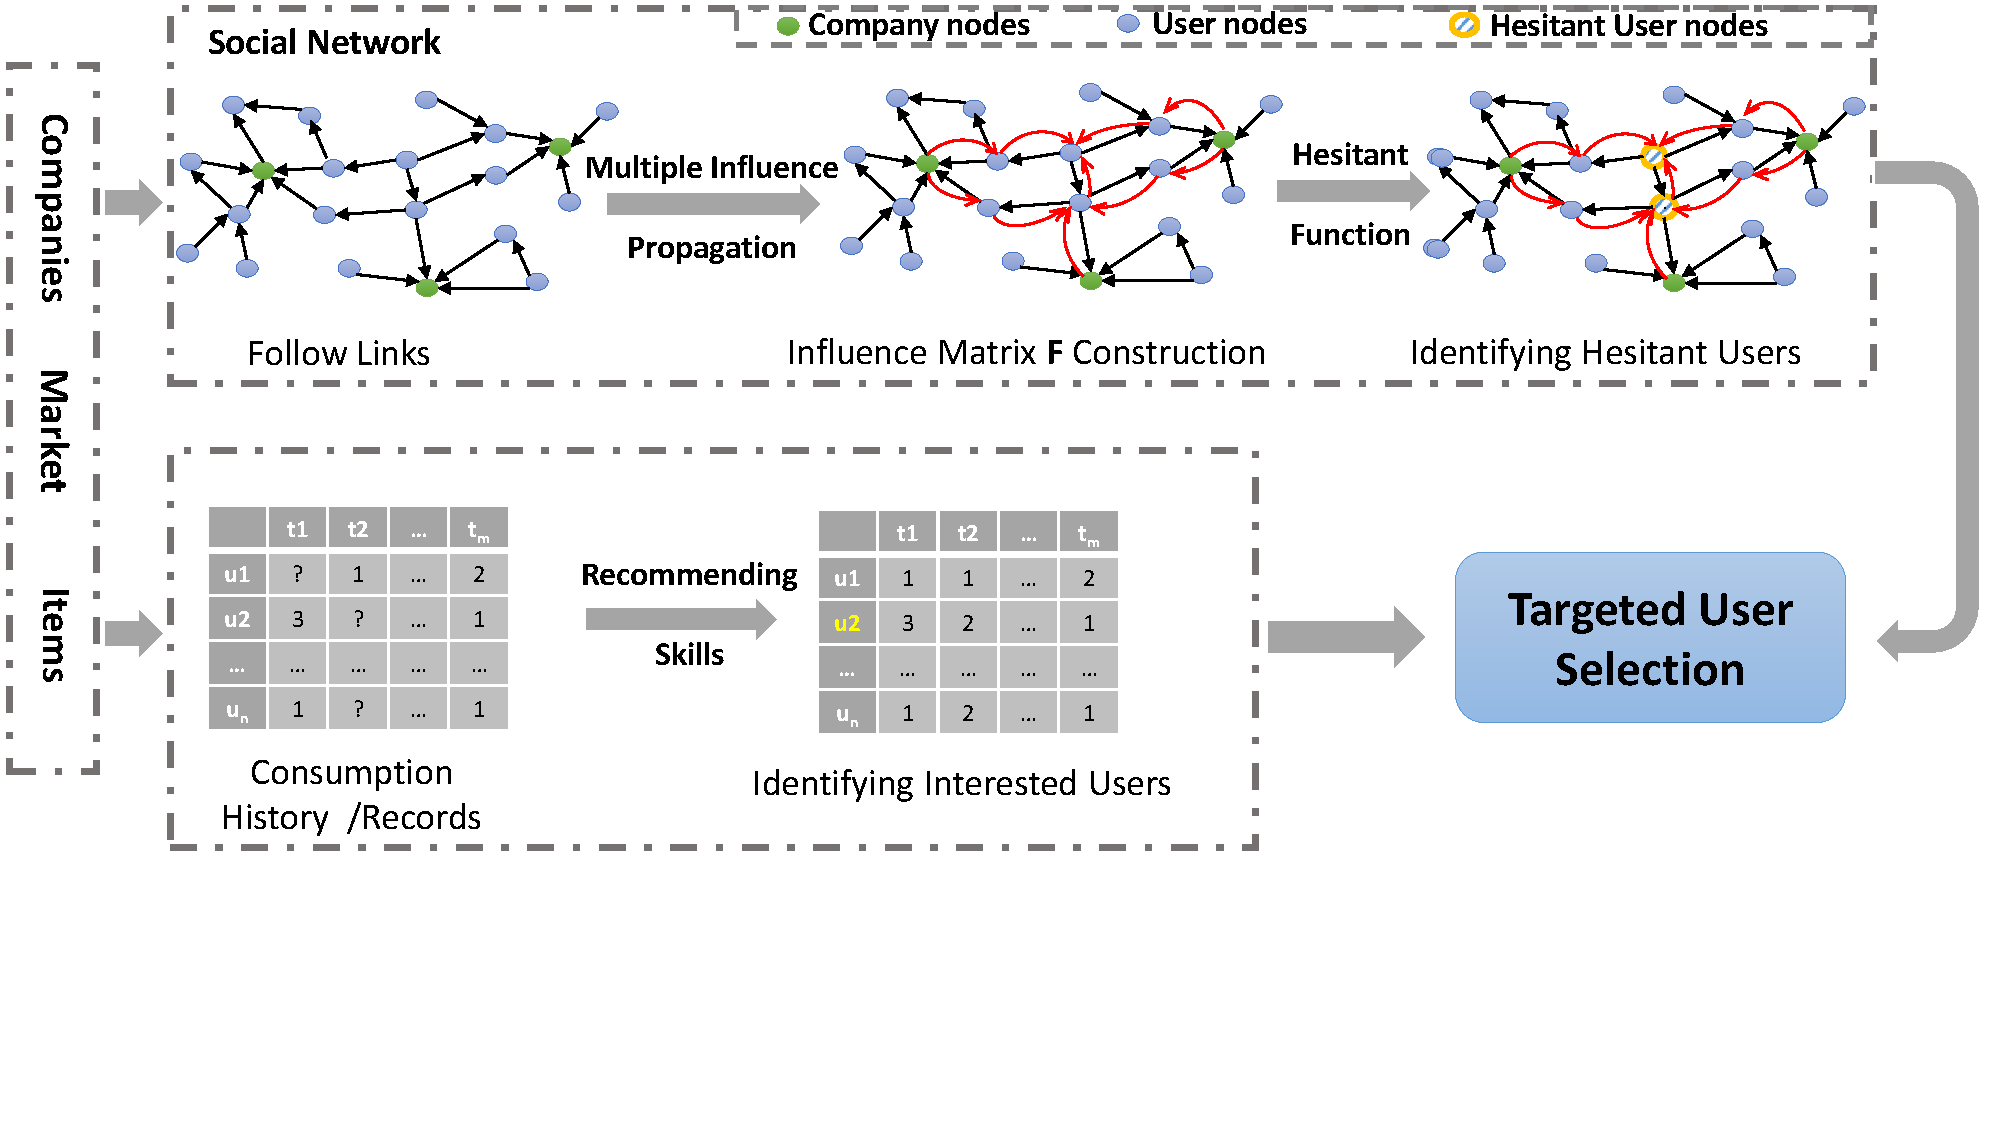
\includegraphics[width=0.85\textwidth]{res/overview.pdf}\\
  \vspace*{-0.5cm}
  \caption{Flowchart of the Framework}\label{fig:overview}
  \vspace*{-0.1cm}
\end{figure}


\vspace*{-0.5cm}
\subsection{Identifying Hesitant Users}
\vspace*{-0.3cm}

In social networks, multiple companies influence each user simultaneously and the users also influence each other. Since we only identify the hesitant users, we focus on the influences of companies on users.

\textbf{Multiple Influence Computation. }
Following the modeling of influence propagation~\cite{ijcai13biaoxiang}, we propose to compute the influence of $j$-th company on each node as:

\vspace*{-0.25cm}
\begin{small}{
\begin{equation}\label{eq:def}
    f_{i\leftarrow j} = \left\{
        \begin{array}{lcl}
            1       &      & {, i \in C_{j}}\\
            0     &      & {, i \in \{C-C_{j}\}}\\
            \sum  _{k\in N(i)} t_{ik} f_{k \leftarrow j}   &      & {, i \in \{V-C\}},
        \end{array}
    \right.
\end{equation}
}\end{small}
\vspace*{-0.25cm}

\noindent
where $N(i)$ is the neighbors of node $i$. In this definition, if the node $i$ belongs to the $j$-th company's official accounts, then $f_{i\leftarrow j} = 1$,which means a company always influence its official accounts; if $i$ belongs to the other companies' official accounts, we assign $f_{i\leftarrow j} = 0$ for the reason that the company's official accounts is hard to be influenced by other companies; if $i$ represents a user, we assign the $f_{i\leftarrow j}$ to the sum of the influence of $j$-th company  on user $i$'s neighbors.

Based on the definition above, we define an influence matrix $\mathbf{F}_{|V| \times |C|}$, where the first $c$ rows represent the company nodes and the remaining $|U|$ rows represent user nodes; the $j$-th column represents the $j$-th company's influence on nodes. 
We propose the MIP (Multiple Influence Propagation) algorithm to construct  $\mathbf{F} = [f_{ij}]_{|V| \times |C|}$, and
Alg.~\ref{alg:mip} shows the details of the MIP. 
There are 4 steps: (1) Initialize the  $\mathbf{F} ^{0}$ (lines 1-7 in Alg.~\ref{alg:mip}); (2) Multiple influences propagation (line 9 in Alg.~\ref{alg:mip}); (3) Reset the companies' influences (lines 10-15 in Alg.~\ref{alg:mip}); (4) Repeat step 2 and 3 until $\mathbf{F}$ converges (lines 8-16 in Alg.~\ref{alg:mip}).
We should note that step 3 is critical: Instead of letting the company nodes' influences ``fade away'', we reset their values to the entries in $\mathbf{F} ^{0}$, so the influence probability mass is concentrated on these company nodes.
\vspace*{-0.15cm}
\begin{algorithm}[tbh]
\SetAlFnt{\footnotesize} %% \scriptsize
\caption{The $MIP$ algorithm} \label{alg:mip}
\vspace*{-0.15cm}
\begin{multicols}{2}
\KwIn{$\textbf{G}=({V},{E},T)$, where $V=C\cup U$}
\KwOut{$\mathbf{F}_{|V| \times |C|}$}
//initialize $\mathbf{F}^{0}$\;
\ForEach {$i\in V$} {
    \For{$j = 1$ \emph{\KwTo} $|C|$}{
        \If{$i \in C_{j}$} {
            $f_{ij}=1$\;
        }
        \Else{
            $f_{ij}=0$\;
        }
    }
}
%\SetAlgoLined
\Repeat{$\mathbf{F}$ converges}{
    $\mathbf{F}~=~T~\mathbf{F}$ \;
    \ForEach {$i \in C$} {
        \For{$j = 1$ \emph{\KwTo} $|C|$}{
            \If{$i \in C_{j}$} {
                $f_{ij}=1$\;
            }
            \Else{
                $f_{ij}=0$\;
            }
        }
    }
}
\textbf{Return}{~$\mathbf{F}$}\;
\end{multicols}
\vspace*{-0.05cm}
\end{algorithm}
\vspace*{-0.15cm}

Next, we analyze the convergence of the computation of influence matrix $\mathbf{F}$. For better presentation, we split $\mathbf{F}$ after the $c$-th row into  2 sub-matrices and split $T$ after the $c$-th row and the $c$-th column into 4 sub-matrices, namely,

\vspace*{-0.25cm}
\begin{small}
\begin{equation*}
    \mathbf{F} = \left[
        \begin{aligned}
          \mathbf{F}_c~~~\\
          \mathbf{F}_{|U|}\\
        \end{aligned}
    \right], ~~~
    T =
    \left[
        \begin{aligned}
            T_{cc}~~~~~~~T_{c{|U|}}~~~\\
            T_{{|U|}c}~~~~T_{{|U|}{|U|}}\\
        \end{aligned}
    \right] .
\end{equation*}\end{small}
\vspace*{-0.25cm}

Thus, step 2 (line 8 in Alg.~\ref{alg:mip}) can be rewritten  as follows:

\vspace*{-0.3cm}
\begin{small}
 \begin{equation*}
    \left[
        \begin{aligned}
          \mathbf{F}_c~~~\\
          \mathbf{F}_{|U|}\\
        \end{aligned}
    \right]
    =
    \left[
        \begin{aligned}
            T_{cc}~~~~~~~T_{c{|U|}}~~~\\
            T_{{|U|}c}~~~~T_{{|U|}{|U|}}\\
        \end{aligned}
    \right]
    \left[
        \begin{aligned}
          \mathbf{F}_c~~~\\
          \mathbf{F}_{|U|}\\
        \end{aligned}
    \right] .
\end{equation*}\end{small}
\vspace*{-0.3cm}

Notice that $\mathbf{F}_c$ never really changes since it is reset after each iteration, and we are solely interested in $\mathbf{F}_{|U|}$.  Obviously, $\mathbf{F}_{|U|} =  T_{{|U|}c}~\mathbf{F}_c +  T_{{|U|}{|U|}} ~ \mathbf{F}_{|U|}$, which leads to
$\mathbf{F}_{|U|} = \lim _{t\rightarrow \infty}  T_{{|U|}{|U|}} ^{t} ~ \mathbf{F}_{|U|} ^{0} + [\sum _{i=1}^{t}
T_{{|U|}{|U|}}^{i-1}]~T_{{|U|}c} ~ \mathbf{F}_c ^{0}$, where $\mathbf{F}_c ^{0}$ and $\mathbf{F}_{|U|} ^{0}$ are the top $c$ rows and the remaining ${|U|}$ rows of the initial $\mathbf{F}$.  According to step 1, we know that $\mathbf{F}_c ^{0} = \mathbf{0}$.
It's obvious that $\mathbf{F}_{|U|} = (I-T_{{|U|}{|U|}})^{-1}~T_{{|U|}c}~\mathbf{F}_c$ is the fixed point. Therefore, the iterative algorithm converges to the unique fixed point.

\textbf{Hesitant Function $H(u)$. }
Based on $\mathbf{F} _{|U| \times |C|}$ (the remaining $|U|$ rows of  $\mathbf{F} _{|V| \times |C|}$), we use a hesitant function $H(u)$ to measure the user hesitancy and identify the hesitant users (like $u_3$, not $u_1$ and $u_2$ in the example of Introduction). %The hesitant function $H(u)$ could measure the hesitancy of user $u$.
The higher of the value $H(u)$, the higher the ``degree of hesitancy'' of the user $u$. If the value $H(u)$ is very low, that means the user $u$ is influenced deeply by some company.
In this part, we introduce two different hesitant functions and  compare their performance in the experiments.
The first $H_{E}(u)$ is transferred from the information entropy~\cite{pang2006introduction} and the second $H_{D}(u)$ is transferred from the information diversity~\cite{tang2014diversified}; their formulations are as below:

\vspace*{-0.3cm}
\begin{small}{
$$H_{E}(u)= \sum _{j=1} ^{|C|} (- f_{uj}\log _{|C|} f_{uj}),~~~H_{D}(u)=\sum _{j=1} ^{|C|} \frac{f_{uj}} {1+f_{uj}}.$$
}\end{small}
\vspace*{-0.3cm}

Now we could recognize the hesitant nodes by using the hesitant functions.
Please note that other rational functions $H(u)$ are also acceptable, such as the Gini index~\cite{pang2006introduction}.



\vspace*{-0.3cm}
\subsection{Identifying Interested Users}
\vspace*{-0.2cm}
Besides measuring the user hesitancy, another key point for selecting targeted users is to measure the user interest, i.e., users' preference on a product and how likely users would consume the product.
Many proposed recommendation methods estimate a utility function $r(u,t)$ to measure the user $u$'s interest on item $t$ and predict how the $u$ will like $t$~\cite{cf2009survey}. 
Since the focus of this paper is not to devise more sophisticated recommendation methods, we choose the two existing methods of \emph{collaborative filtering}: item-based collaborative filtering (ICF)~\cite{deshpande2004item} and user-based collaborative filtering (UCF)~\cite{cf2009survey}.  The corresponding formulas are as below:

\vspace*{-0.4cm}
\begin{small}{
$$ r(u,t)_{ICF} = \frac {\sum _{k \in M(u)}  sim(k,t)~ r_{uk}} {\sum _{k \in M(u)} sim(k,t)}, ~~~~
r(u,t)_{UCF} =  \frac {\sum _{v \in S(u)} sim(u,v)~ r_{vt}} {\sum _{v\in S(u)} sim(u,v) },$$
}\end{small} \vspace*{-0.4cm}

\noindent
where $M(u)$ is the items that user $u$  have consumed, $S(u)$ is the users who are most similar to $u$, $sim(k,t)$  is the similarity between items $k$ and $t$, and $sim(u,v)$  is the similarity between users $u$ and $v$; both of them are computed based on the user's past consumption behaviors $R_{|U| \times |M|}$.  In this paper, we choose the Jaccard measure to calculate the similarities, and the formulas are as below:

\vspace*{-0.3cm}
\begin{small}{
$$sim(k,t) =  \frac {\mathbb{U}_{k} \cap \mathbb{U}_{t}} {\mathbb{U}_{k} \cup \mathbb{U}_{t}} ,~~~~~~~~~
 sim(u,v) = \frac {\mathbb{I}_{u} \cap \mathbb{I}_{v}}{\mathbb{I}_{u} \cup \mathbb{I}_{v}} ,$$
}\end{small} \vspace*{-0.3cm}

\noindent
where $\mathbb{U}_{k}$ and $\mathbb{U}_{t}$ represent the users who have consumed $k$ and $t$, respectively; $\mathbb{I}_{u}$ and $\mathbb{I}_{v}$ represent the items which have been consumed by $u$ and $v$,respectively.

Without loss of generality, we use ICF and UCF to select users with highest values as the interested users, and we will experimentally compare the performance of them.


\vspace*{-0.4cm}
\subsection{Targeted User Selection}
\vspace*{-0.2cm}
According to the illustrations above, we could compute the $H(u)$ and $r(u,t)$ to measure the user hesitancy and the user interest. Finally, we combine the two characters of user and propose the function $P(u,t)$ to measure the overall quality of each user.  The final function $P(u,t)$ is as follows:
\vspace*{-0.3cm}
\begin{small}{
\begin{equation}\label{eq:finalP}
P(u,t) =  \eta \frac {H(u)}{\bar{H}(u)} + ( 1 - \eta ) \frac { r(u,t)} {\bar{r}(u,t)} ~,
\end{equation}
}\end{small} \vspace*{-0.4cm}

\noindent
where $\eta$  is used to balance the effect of the hesitancy and the interest, and the $\bar{H}(u)$ and $\bar{r}(u,t)$ are the maximum $H(u)$ and $r(u,t)$, respectively. 
The smaller the $\eta$, the more we pay on the interest measure. When $\eta$ reduces to $0$, the function only considers the user interests, thus the approach turns to traditional collaborative filterings. 

Finally, a set $S$ of $K$ users with the highest value of $P(u,t)$ will be selected as the targeted customers for the given company when it wants to market the product $t$.


%%%%%%%%%%%%%%%%%%%%%%%% Experiments %%%%%%%%%%%%%%%%%%%%%%%%%%%
\vspace*{-0.3cm}
\section{Experiments}
\vspace*{-0.35cm}
\subsection{Experimental Setup}
\vspace*{-0.3cm}
The experiments are conducted on real-world social datasets: \emph{Weibo} and \emph{Epinions}.

(1) \emph{Weibo}. We crawled from the social media weibo.com, where nodes represent the users or the companies' official accounts, and edges are nodes' followships. When a user posts a message in Weibo, the sending device (e.g., the mobile devices like Samsung Galaxy Note and iPhone5) are also recorded. That is, we can obtain the mobile purchasing behaviors of users by their posted messages. For instance, if a user send messages using Samsung Galaxy Note, we say he is a consumer of Samsung, and then he send another message by using ``Xiaomi 2'', we say the user is also a consumer of Xiaomi\footnote{A user's consumptions/messages using the same mobile device will be integrated into a tuple record(user id, mobile id, number of records).}.
 This data is collected in March 2013. For better illustration, we sample a small network which only contains the verified users and the official accounts of the five($|C|=5$) famous mobile companies (namely, Samsung, Huawei, Xiaomi, HTC and ZTE)~\footnote{As Apple Inc. has none official account in Weibo, our collections does not contain it.}; more specifically, each mobile company contains two or three official accounts(namely, $C_i = 2 ~or ~3$). In this way, we could obtain the consuming records $R$.

(2) \emph{Epinions}. Epinions.com is a well known knowledge sharing and review site. In this site, registered users can submit their personal opinions on some topics such as products, movies or the reviews issued by other users, and assign products or reviews integer ratings from 1 to 5. These ratings and reviews will influence future customers when they are about to decide whether a product is worth buying or a movie is worth watching, and each rating could be regarded as a consumption from a user to an item (product or movie). Every member of Epinions maintains a ``trust'' list which presents a social network of trust relationships between users. To use this dataset, we select the $|C|=5$ influential users (having the most followers) and treat them as the companies (i.e., $|C_i| = 1$ for this dataset as each selected user/company has only one account). Then, the items are the opinions/products shown by each user/company.

\begin{table}[thb]
%\scriptsize %\small \footnotesize \tiny \scriptsize
\centering
\caption{Statistics of the Datasets.}\label{table:datasets}
\vspace*{-0.3cm}
%\begin{center}
\begin{tabular*}{0.75\textwidth}{l|rrrr}
  \cline{1-5}
  % after \\: \hline or \cline{col1-col2} \cline{col3-col4} ...
  Data &~ \#Nodes &~ \#Items &~ \#Social Edges &~ \#Consumptions \\
  \cline{1-5}
  Weibo  &~ 140,876 &~ 89   &~  1,792,835 &~ 2,822,315 \\
  % WeiboSample  &~ 2571+9 &~ 72   &~ 6404+1730=8134 &~ 194665 \\
 % \cline{1-5}
  Epinions &~ 49,290 &~ 139,738 &~ 487,183 &~ 664,824 \\
  \cline{1-5}
\end{tabular*}
%\end{center}
%\vspace*{-0.2cm}
\end{table}

Detailed information about the two datasets can be found in Table~\ref{table:datasets}. 
For each dataset, we split it into a training set and a test set, by selecting the first 80 percentage of the consumptions for training and the remaining ones to be part of the test set. In this way, we could validate the performance of our methods on the test set. 


\vspace*{-0.35cm}
\subsection{The Correlation Analysis}
\vspace*{-0.3cm}
In this subsection, we use \emph{Weibo} as an example to show the strong correlations between social follow-links (between users and companies) and users' consumption behaviors.

First, we calculate the product (mobile) adoption rate of each company's followers and the results are shown in Fig.~\ref{fig:casestudya}. From each subfigure (with respect to one company), we could observe that most of the followers adopt each company's products (Due to space limitation, we omit the result on ZTE). For instance, the first subfigure shows the product adoption rate of Xiaomi's followers, where 50\% of these followers use the products (cellphones) produced by Xiaomi. Then, we calculate the following rate of the companies' consumers (the percentage of each company's consumers that follow this given company) and the results are shown in Fig.~\ref{fig:casestudyb}. We can see that most of each company's consumers incline to follow this company's accounts. For instance, the first subfigure of Fig.~\ref{fig:casestudyb} shows that among the users who consumed Xiaomi's products, 71\% of them followed Xiaomi's official accounts in Weibo, while only 13\%, 8\%, 4\% of them followed the official accounts of HTC, Huawei and Samsung, respectively.

The above results demonstrate that there exists an obvious correlation between the social relations (influence) and the users' consumption behaviors. Thus, it is necessary to exploit the social influence for targeted marketing. More deeply understanding will be shown in the following subsection.

\begin{figure}[t]
  \vspace*{-0.3cm}
  \begin{minipage}[t]{\textwidth}
    \centering
    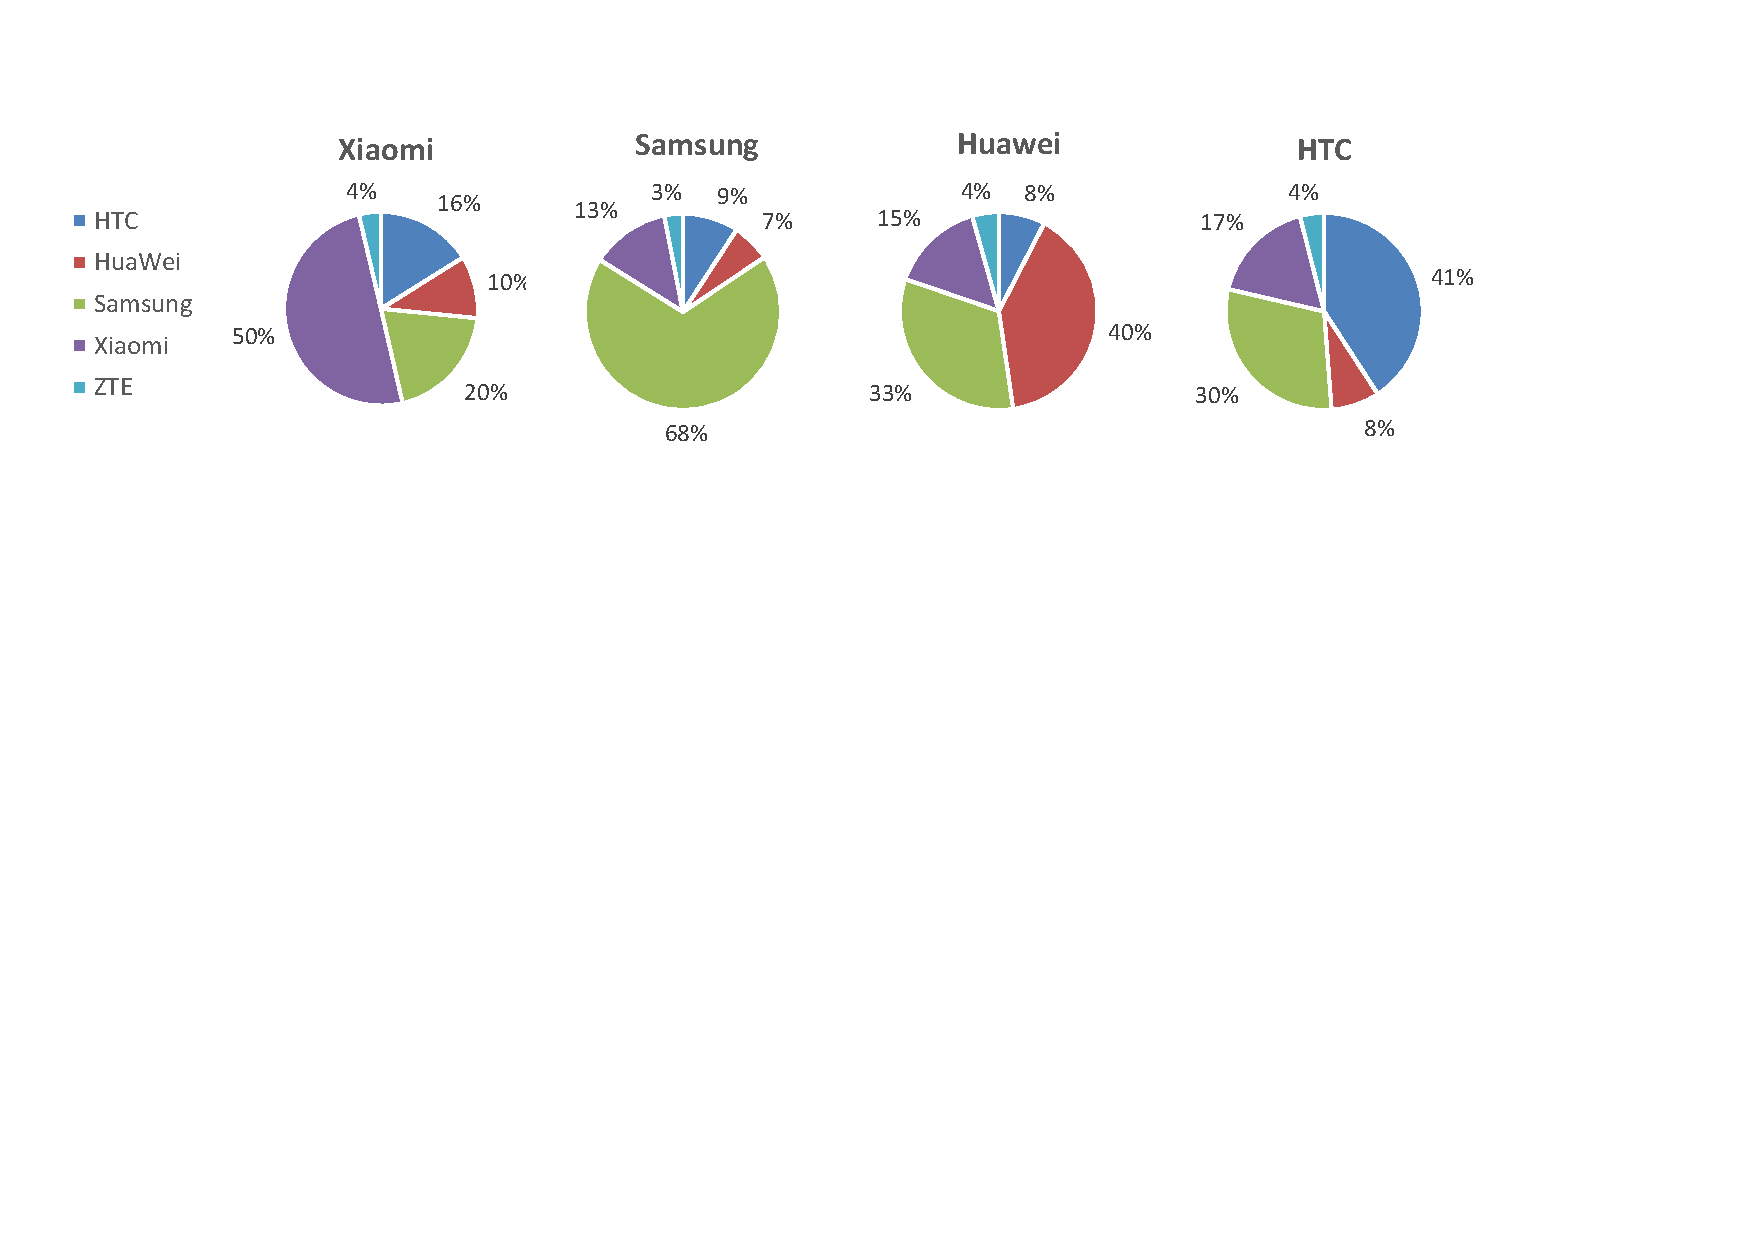
\includegraphics[width=0.86\textwidth]{res/isu_c_correlation_a_pie.pdf}\\
    \vspace*{-0.6cm}
    \caption{Product Adoption Rate of the Company's Followers}\label{fig:casestudya}
  \end{minipage}%%

  \vspace*{-0.2cm}
  \begin{minipage}[t]{\linewidth}
  \centering
  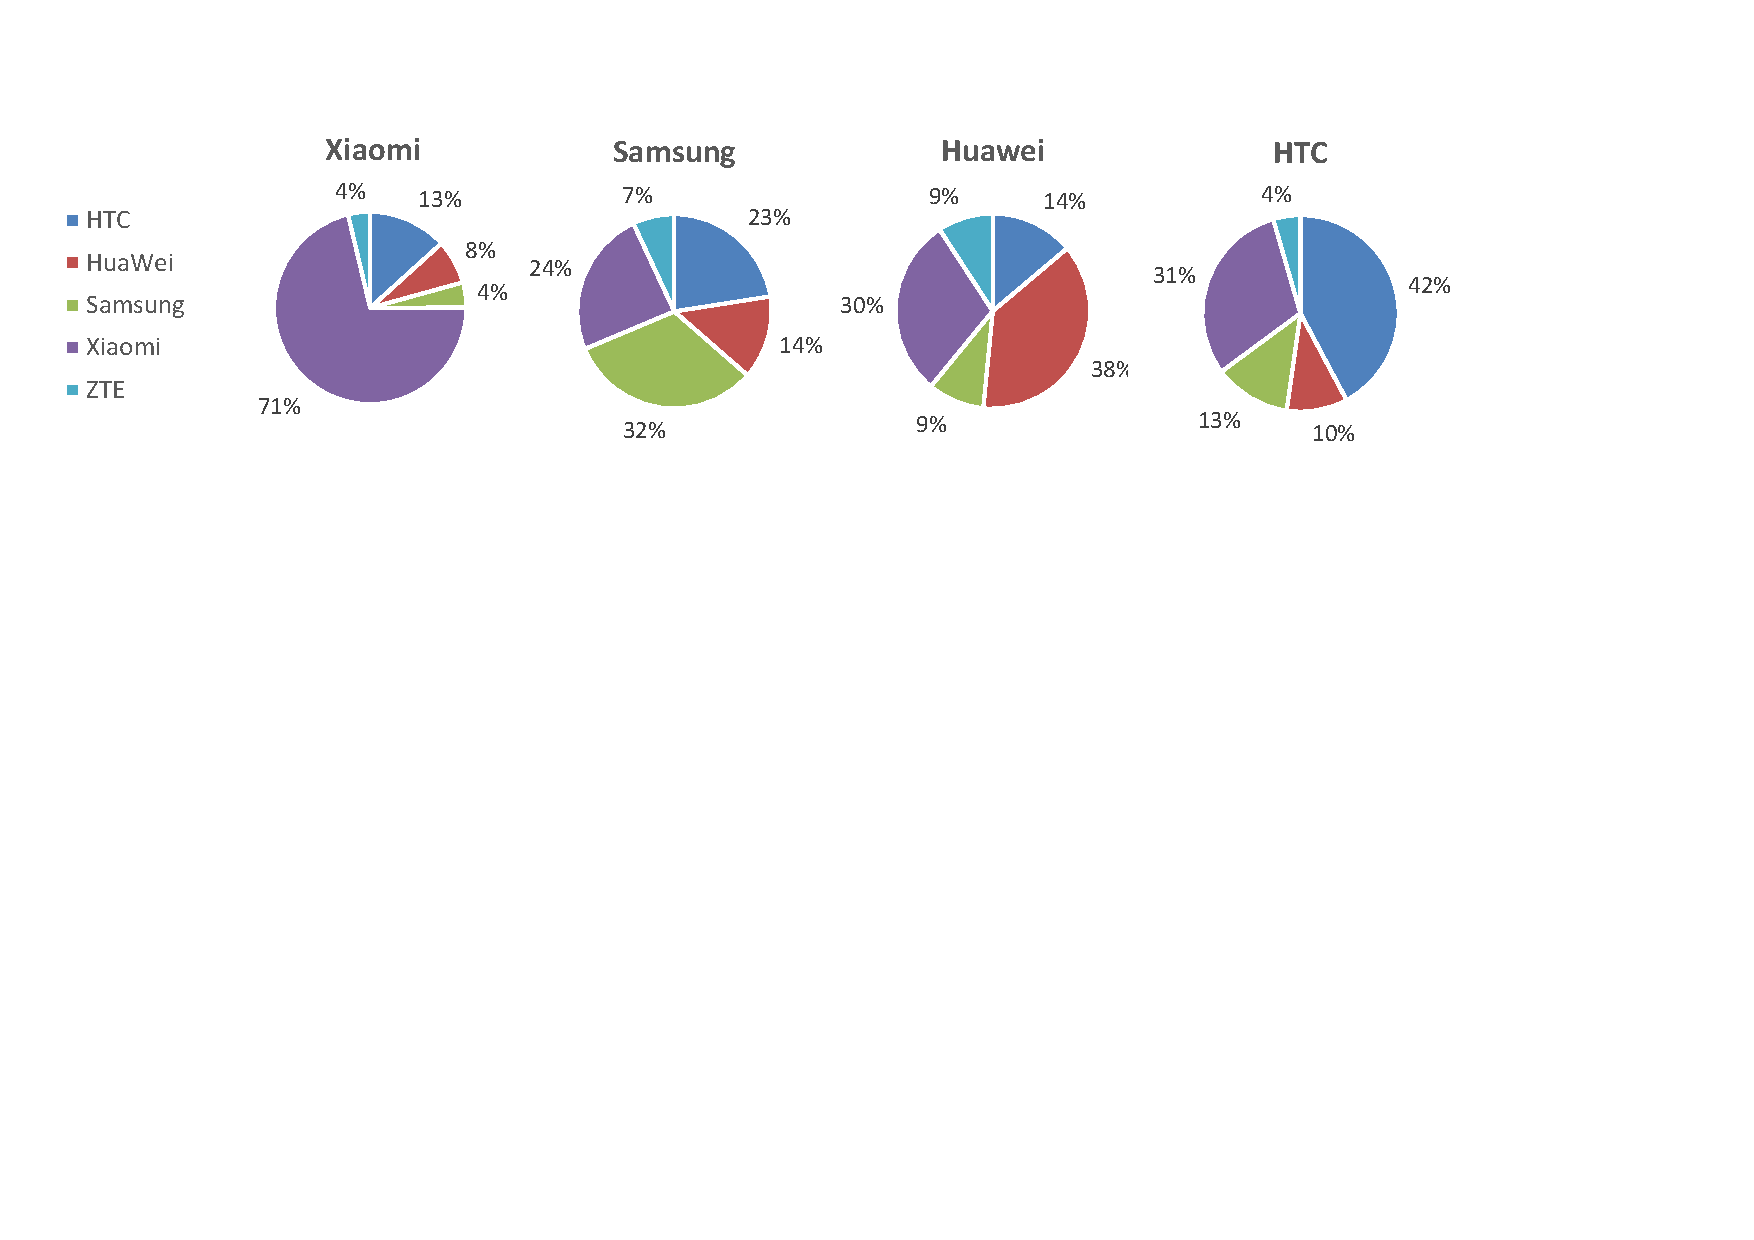
\includegraphics[width=0.86\textwidth]{res/isu_c_correlation_b_pie.pdf}\\
   \vspace*{-0.6cm}
  \caption{Following Rate of the Companies' Consumers}\label{fig:casestudyb}
  \end{minipage}
  \vspace*{-0.25cm}
\end{figure}




\vspace*{-0.4cm}
\subsection{Evaluation of the MIP algorithm}
\vspace*{-0.3cm}
We further validate the assumption (the users who are deeply influenced by a company have much higher probability to choose the company's new product) by our MIP algorithm, and then demonstrate the performance of MIP.

\textbf{Assumption Validation based on MIP.} We first use MIP to compute the influence matrix $\mathbf{F}_{|V| \times |C|}$ on the training data. Then we select the top $K$ users who have been deeply influenced by each company $j=1,2,...,5$, and compute the adoption (buy or rate the company's products) rate of these deeply influenced users on the test data, i.e., InfRate. We compare this InfRate with the average adoption rate of all users, i.e., AvgRate. The results are shown in Fig.~\ref{fig:assumptionvalide}, where we set $K=30$ for \emph{Weibo} and $K=500$ for Epinion due to the different data sparsity. Specifically, the left and middle subfigures of Fig.~\ref{fig:assumptionvalide} are the comparison results on \emph{Weibo} and Epinion, and the right subfigure shows the Growth Rate of InfRate compared to AvgRate. For instance, On \emph{Weibo}, the users who are deeply influenced by HTC (Company ID 1 in the right subfigure) have 60\% probability to choose HTC's products (the left subfigure) and this rate is 16 times higher than AvgRate (the right subfigure). Once again, we could conclude that the users who are deeply influenced by a company have higher probability to choose the company's new product and lower probability to choose the competitors'. Hence, when conducting targeted marketing, the company should pay more attention to the hesitant customers, since the deeply influenced customers will choose the influencer's product.

\begin{figure}[htb]
  \centering
  % Requires \usepackage{graphicx}
  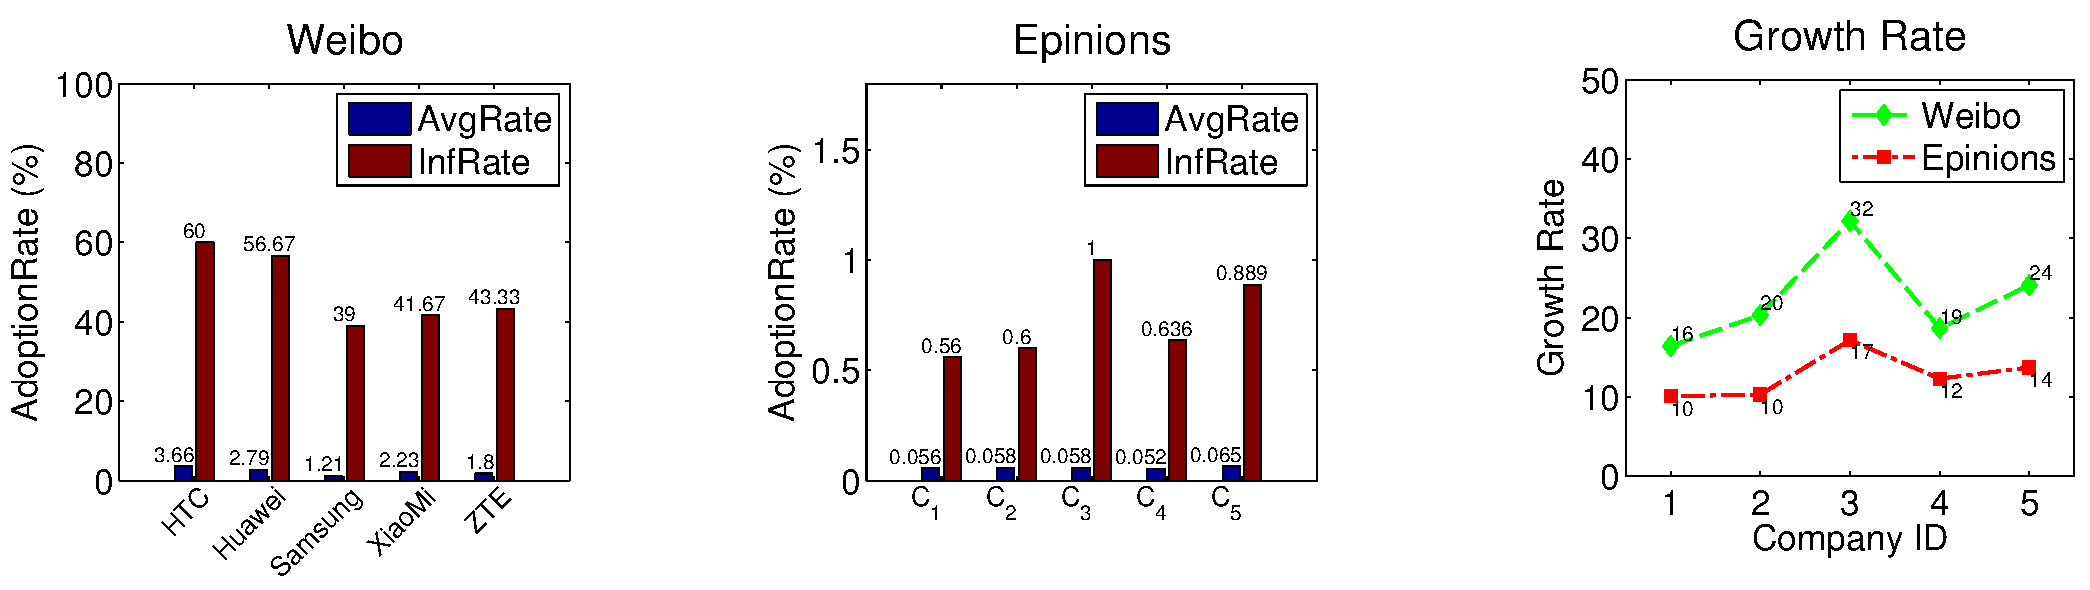
\includegraphics[width=0.9\textwidth]{res/isu_b_f2.pdf}\\
  \vspace*{-0.65cm}
  \caption{Adoption Rate of the deeply influenced users}\label{fig:assumptionvalide}
 \vspace*{-0.15cm}
\end{figure}


\textbf{Efficiency and Effectiveness of MIP. } Although several influence models (such as IC~\cite{kempe2003maximizing}, LT~\cite{granovetter1978threshold} and Linear~\cite{ijcai13biaoxiang}) have been proposed to compute the influence of one node to another, none of them are efficient or suitable for measuring the influences from multiple companies on users. Without loss of generality, we use the recently proposed Linear model (which is both efficient and effective) as the baseline of our MIP algorithm, and the parameter settings (including the entries in $T$) are same to that in~\cite{ijcai13biaoxiang}.

Specifically, we first use MIP and Linear, respectively, to get $\mathbf{F}$, and then compute the users' hesitant value $H(u)$. We run the process 100 times for different number of companies (i.e., $|C|$ equals to 1,2,..., or 5) and then compare the average runtime of the two methods. The results shown in Fig.~\ref{fig:runtime} demonstrate that MIP is much more efficient and is also invariant to the number of companies. In addition, we compare the average hesitant values ($H(u)^{MIP}$ and $H(u)^{Linear}$ ) of the randomly selected 25 nodes, and then compute the difference rate $({H(u)^{MIP}- H(i)^{Linear}} )/ { H(u)^{Linear} }$ under the $|C|=3$. This result is shown in Fig.~\ref{fig:hesitantEntropy}. The results illustrate that the value of $H(u)^{MIP}$ and $H(u)^{Linear}$ are very similar as the difference rate are almost less than 0.05. In other words, MIP has the similar ability to measure the social influence prorogation process as Linear, while MIP is much more efficient for computing the influences from multiple companies on users.

\begin{figure}[htb]
 %\vspace*{-0.3cm}
\begin{minipage}[t]{0.5\linewidth}
   \centering
   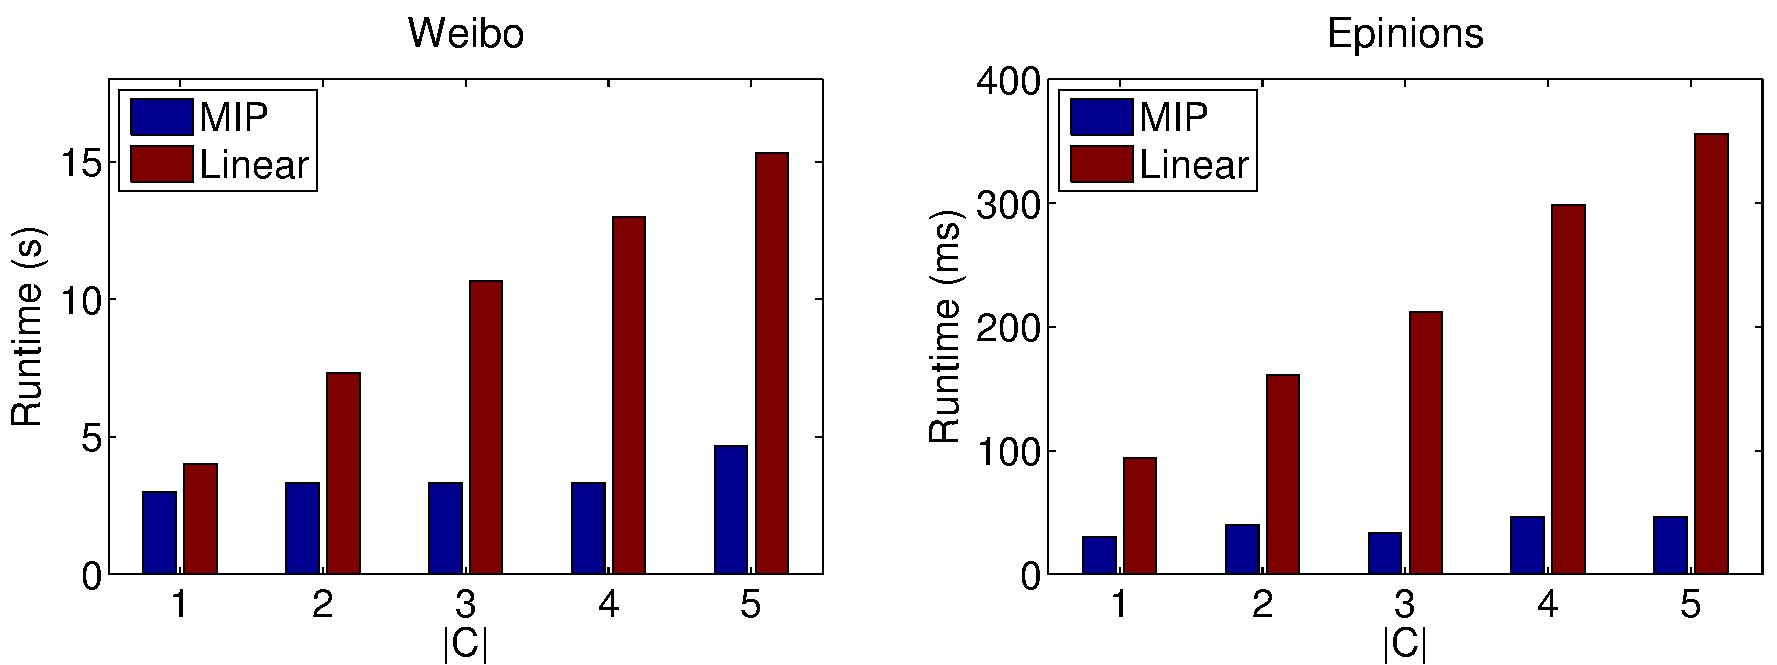
\includegraphics[width=0.95\textwidth]{res/isu_b_runtime.pdf}\\
   \vspace*{-0.4cm}
   \caption{Runtime Comparisons}\label{fig:runtime}
\end{minipage}%%
\begin{minipage}[t]{0.5\linewidth}
   \centering
   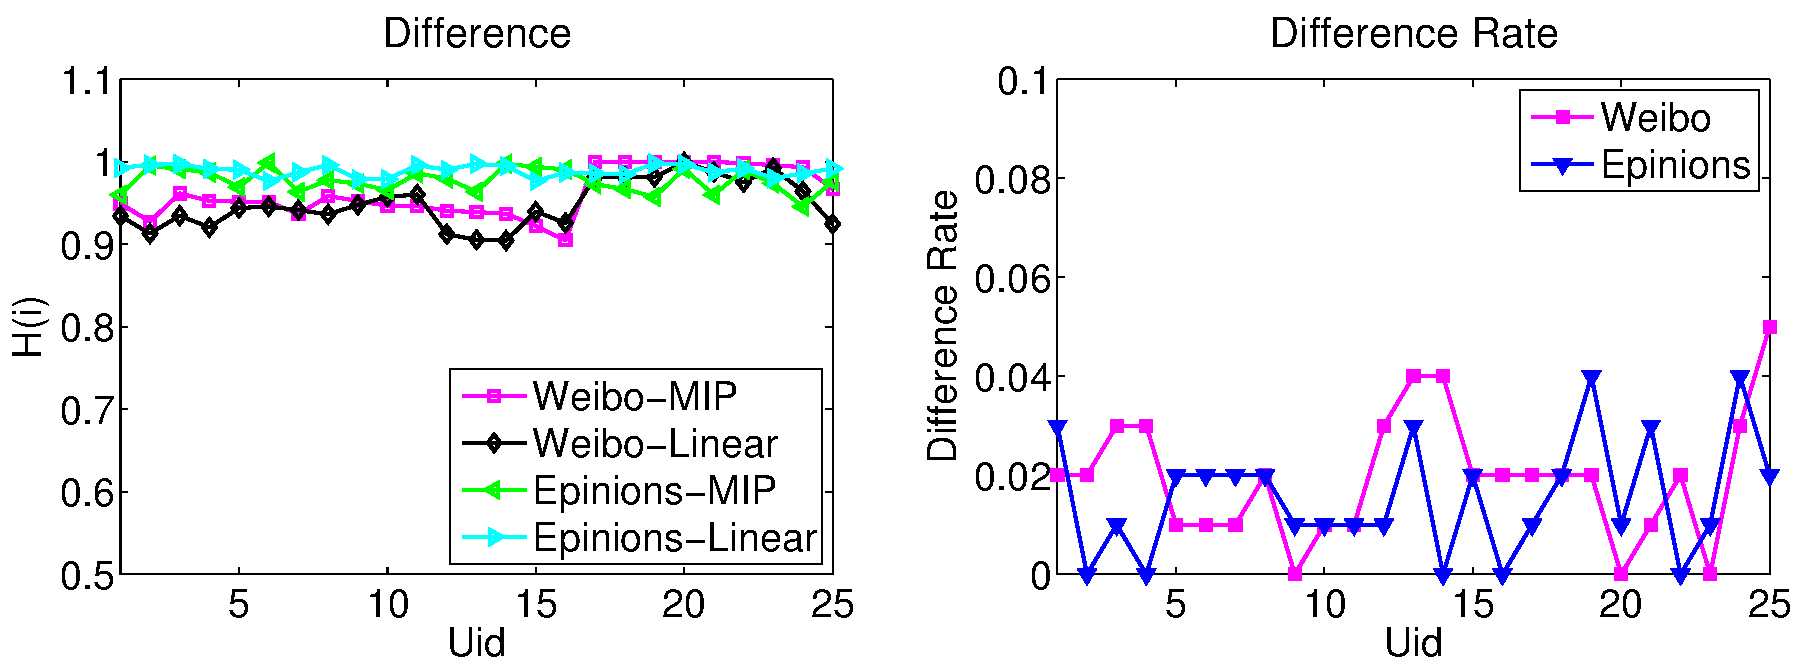
\includegraphics[width=0.95\textwidth]{res/isu_b_entropyRate.pdf}\\
   \vspace*{-0.4cm}
   \caption{$H(u)$ Comparisons}\label{fig:hesitantEntropy}
\end{minipage}
 %  \vspace*{-0.3cm}
\end{figure}

\vspace*{-0.6cm}
\subsection{Evaluation of Function $P(u,t)$}
\vspace*{-0.3cm}
In this subsection, we first show the effects of the parameter $\eta$ for final targeted user selection, and then compare the performance of $P(u,t)$ with two baselines. Finally, we generalize the $P(u,t)$ with different functions of $H(u)$ and $r(u,t)$. 

Specifically, we choose $H_{E}(u)$ to identify hesitant users, and use $r(u,t)_{ICF}$ to identify interested users~(the generality of other functions will be evaluated later). Then the quality function $P(u,t) = \eta H_{E}(u)/ \bar{H}(u) + (1-\eta) r(u,t)_{ICF}/\bar{r}(u,t)_{ICF}$ is used to select targeted users (i.e., IHIC). We select two related benchmarks:
\begin{compactitem}
  \item \textbf{ICF} is short for item-based collaborative filtering, only takes the user interest into consideration. Actually, ICF is a special case of IHIC when $\eta = 0$.
  \item \textbf{IHC} is short for identifying hesitant customers. The IHC method only considers the user hesitancy and is a special case of IHIC when $\eta = 1$ for $P(u,t)$.
\end{compactitem}


\textbf{The Effects of $\eta$. }
We first show whether different values of $\eta$ can help select different targeted customers. For comparison, we first use ICF to identify a targeted user set $S_{ICF}$. Then we change the values of $\eta$ from 0 to 1 with a stepsize of 0.1, and each time  we select another targeted use set $S_{IHIC}$ with the $\eta$ value and compute the Jaccard similarity between the two targeted user sets. 
We also further compute the Jaccard similarity of the consumed items of the selected users. In practice, the size of the targeted user set is set to 30 and the results are averaged over 50 randomly selected items. 
The final results are shown in Fig.~\ref{fig:a1similarity}; we can see that the larger the $\eta$, the bigger the difference between the user sets and the consumption behaviors of the selected targeted users. We conclude that IHIC($P(u,t)$) is able to select different targeted users with different $\eta$, and these users also have different item preferences.
\begin{figure}[ht]
%  \vspace{-0.5cm}
  \centering
  % Requires \usepackage{graphicx}
  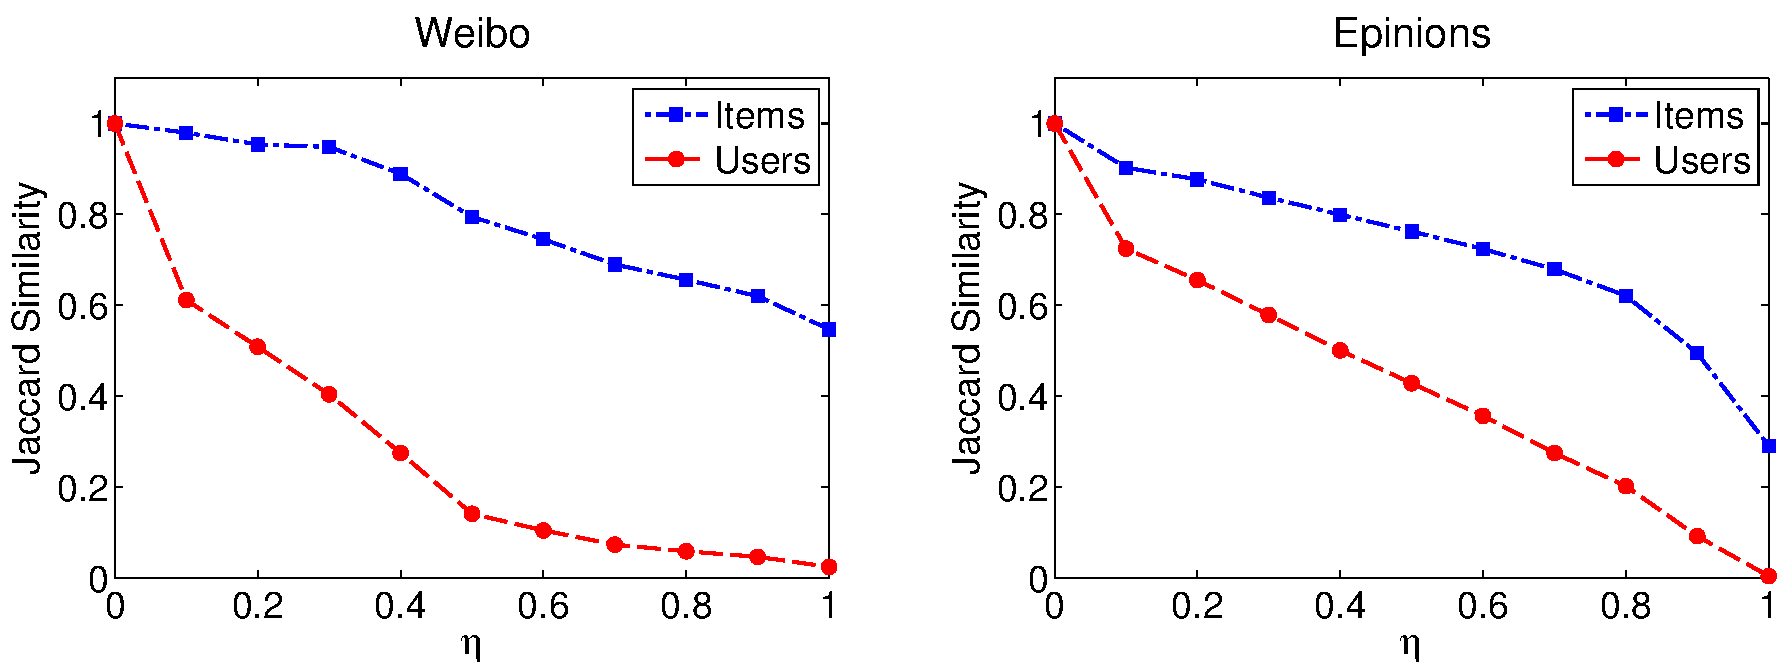
\includegraphics[width=0.6\textwidth]{res/isu_a_similarity.pdf}\\
   \vspace{-0.4cm}
  \caption{The Jaccard Similarity of the user sets and their consumed items}\label{fig:a1similarity}
%  \vspace{-0.2cm}
\end{figure}


\textbf{Performance Comparisons.} For a marketing item, we select the targeted users $S$ on the training data by each method. Then, we compute the precision and recall of $S$ on the test data to measure the performance of these methods, e.g., precision equals to the percentage of these targeted users that consumed the item.

Before detailed comparison with other models, we need to first select the best $\eta$ for our proposed IHIC model. We randomly select 50 items and get the target users by IHIC with different $\eta$ values under different target user size~($|S|=\{10,20,30\}$). 
Fig.~\ref{fig:aprweibo} and Fig.~\ref{fig:aprepinion} show the results on \emph{Weibo} and \emph{Epinions} respectively, which illustrate that the performance (both precision and recall) of IHIC changes with different $\eta$;
 additionally, IHIC could achieve the better performance with some value $\eta \in (0.1, 0.4)$. This implies that we could change the performance of selected targeted users by considering the user hesitancy with different weight($\eta$), and choose the $\eta$ leading to the best performance.


Then, we compare the performances of targeted users with different $|S|$ selected by the three methods (IHIC, ICF, IHC); 
we set $\eta=0.2$ for better performance~\footnote{In fact, the optimum $\eta$  could be estimated by using a validation set.}. Fig.~\ref{fig:aprweibocomp} and Fig.~\ref{fig:aprepinioncomp} show the results of the performance comparisons on \emph{Weibo} and \emph{Epinions} respectively. The results illustrate that the traditional recommendation method ICF not always achieve the best results. Nevertheless, IHIC, which considers both the user interest and hesitancy, usually obtains better performance. This implies that many higher interested users selected by ICF are deeply influenced by another company, and they incline to choose the similar products of the competitor's.
Hence, it's necessary to consider the user hesitancy when conducting product marketing.

\begin{figure}[hbt]
\begin{minipage}[t]{0.5\linewidth}
  \centering
  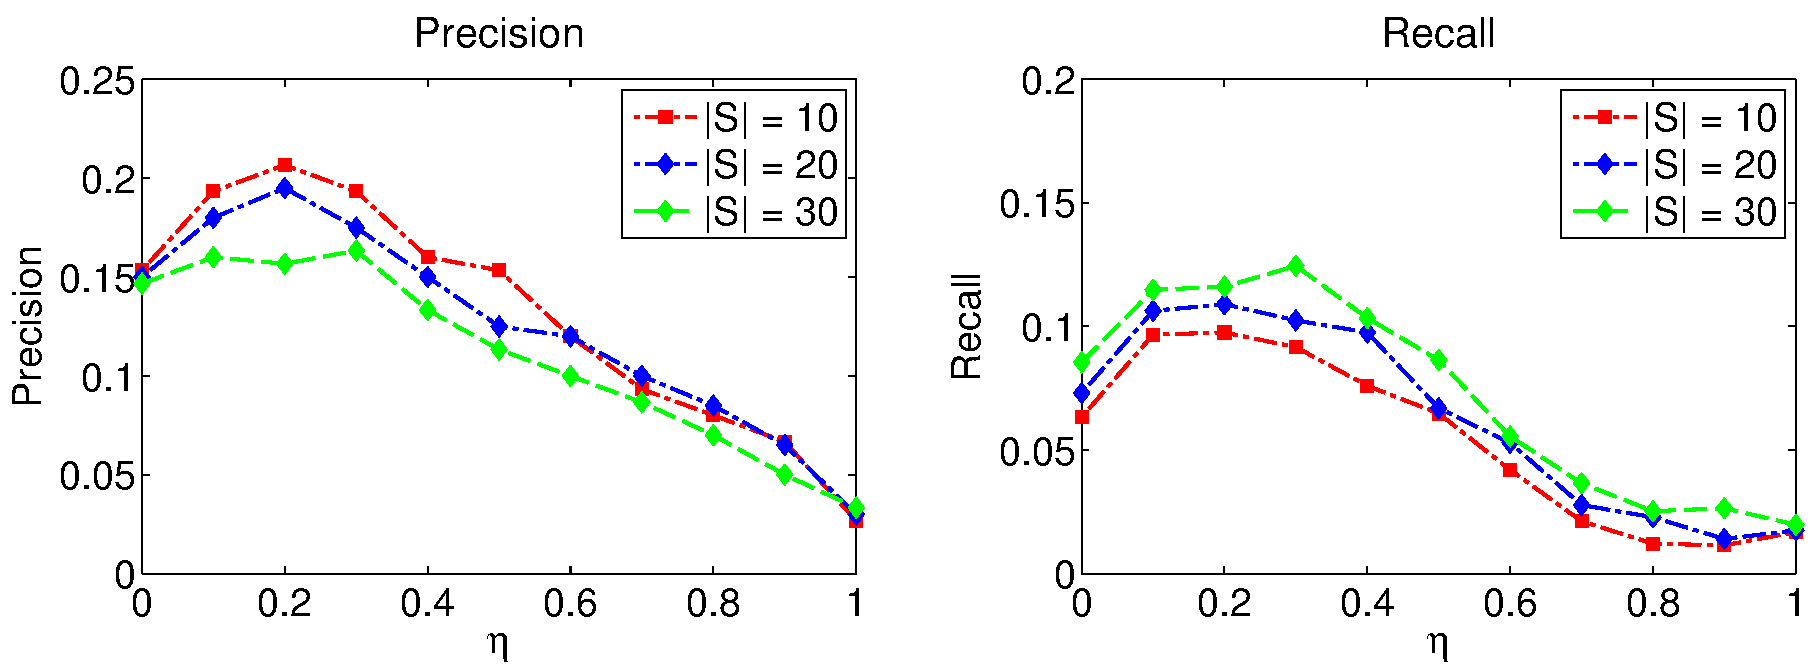
\includegraphics[width=0.95\textwidth]{res/isu_a_pr_weibo.pdf}\\
  \vspace*{-0.4cm}
  \caption{Precision and Recall on \emph{Weibo}} \label{fig:aprweibo}
\end{minipage}%%
\begin{minipage}[t]{0.5\linewidth}
  \centering
  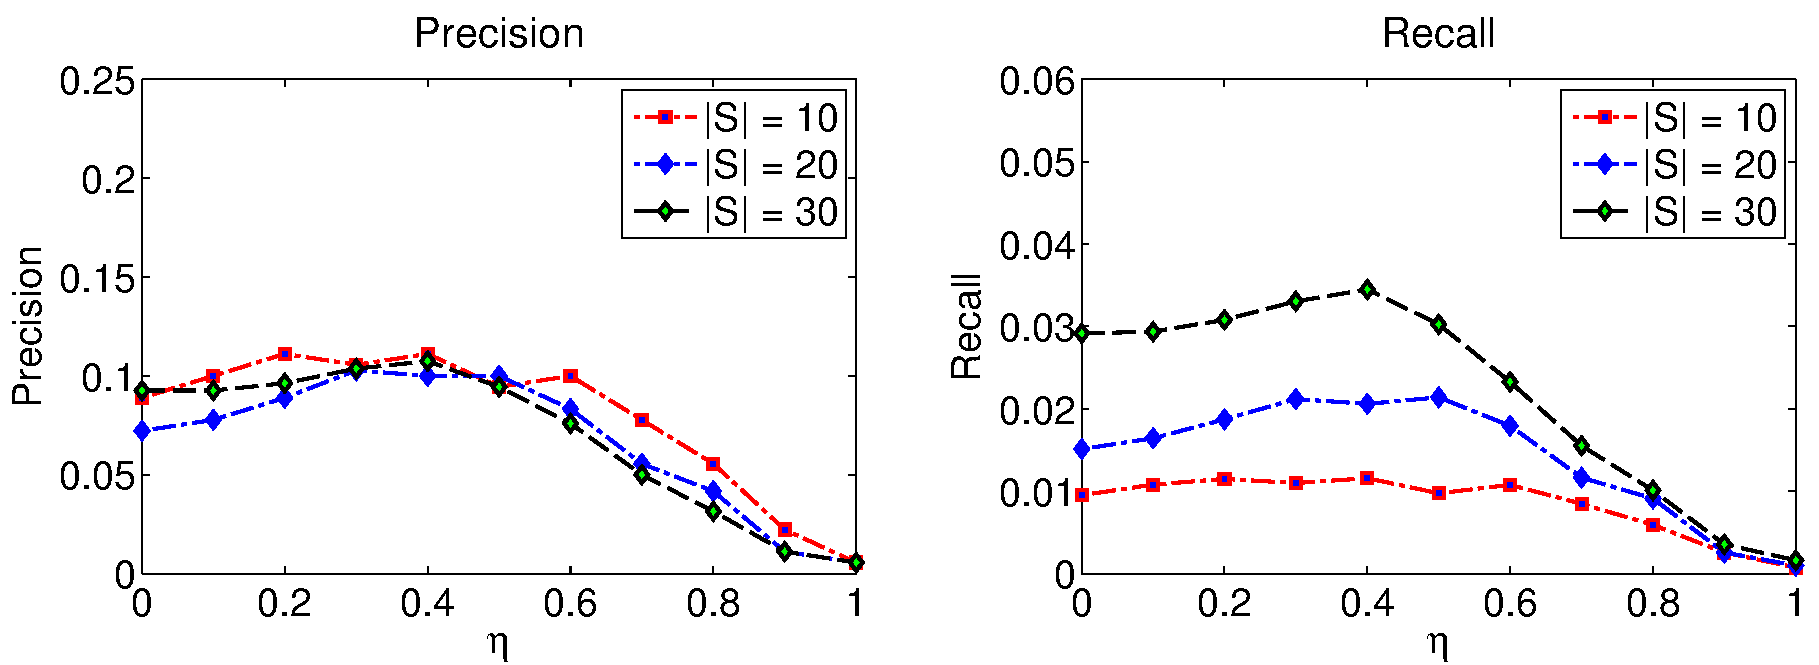
\includegraphics[width=0.95\textwidth]{res/isu_a_pr_epinion.pdf}\\
  \vspace*{-0.4cm}
  \caption{Precision and Recall on \emph{Epinions}} \label{fig:aprepinion}
\end{minipage}
\end{figure}

\begin{figure}[ht]
\begin{minipage}[t]{0.5\linewidth}
  \centering
  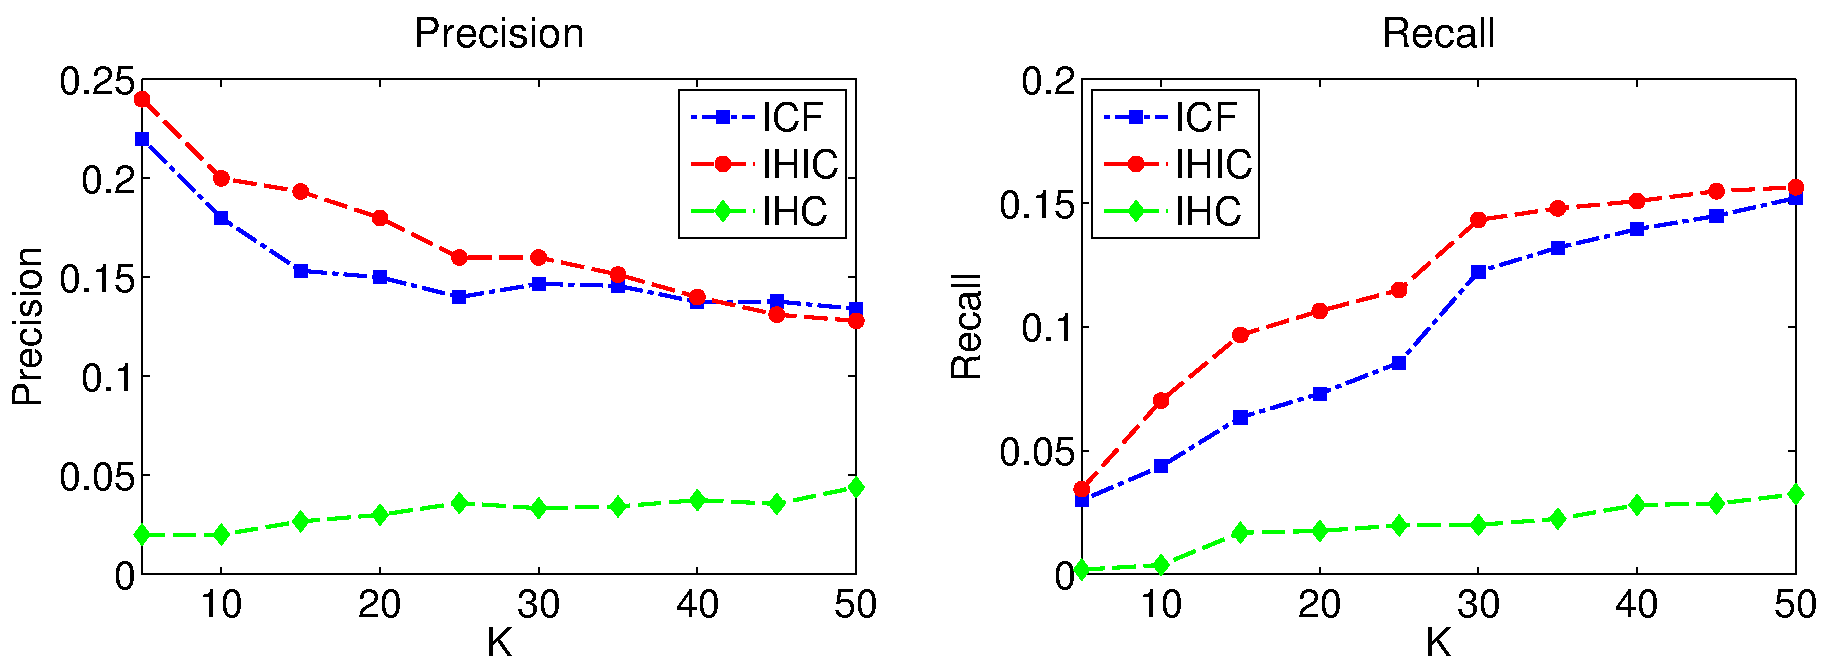
\includegraphics[width=0.95\textwidth]{res/isu_a_pr_weibo_comparison.pdf}\\
  \vspace*{-0.4cm}
  \caption{Comparisons on \emph{Weibo}} \label{fig:aprweibocomp}
\end{minipage}%%
\begin{minipage}[t]{0.5\linewidth}
  \centering
 %\includegraphics[width=2.2in]{fig2.eps}
  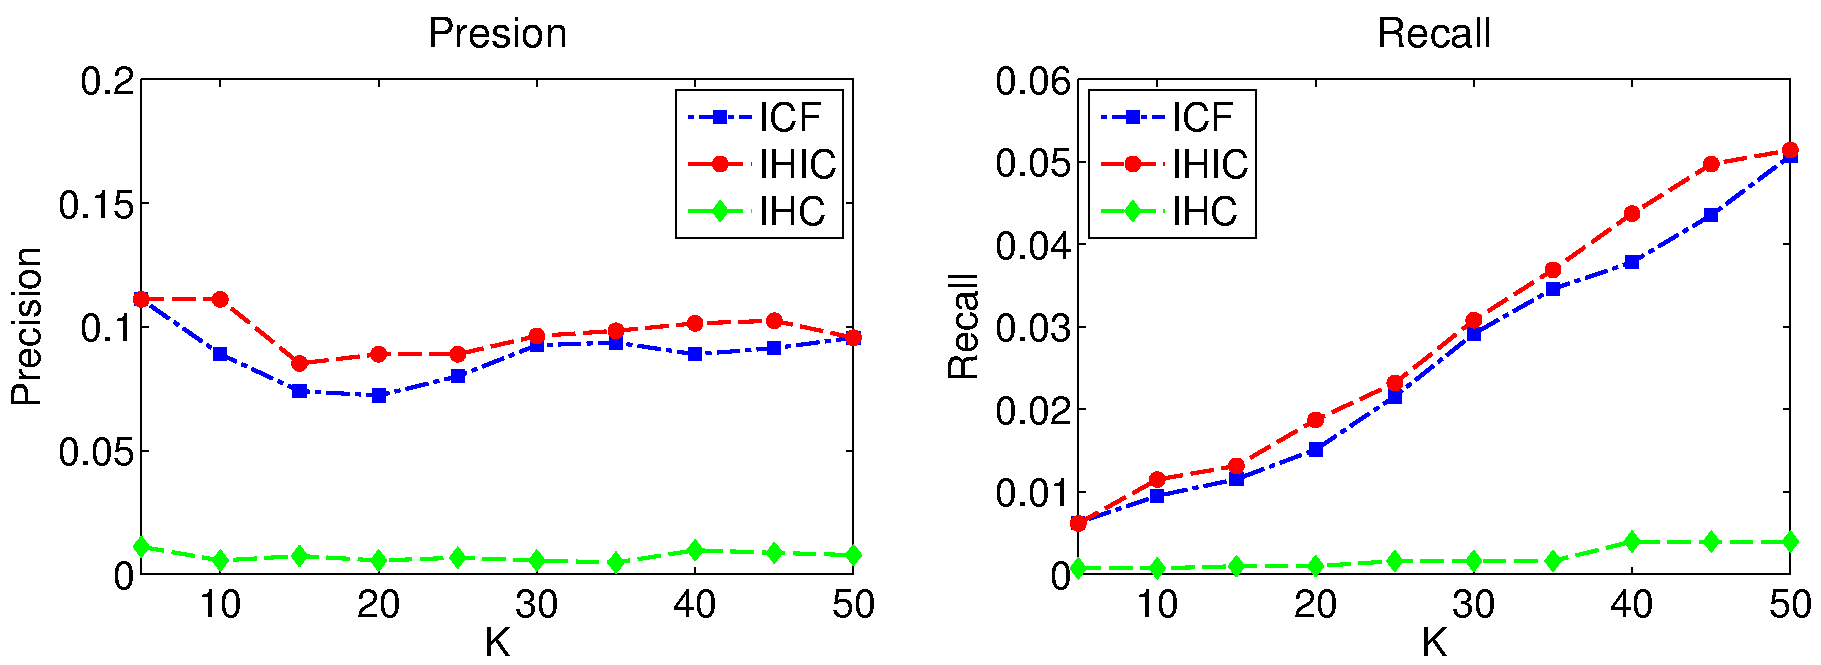
\includegraphics[width=0.95\textwidth]{res/isu_a_pr_epinion_comparison.pdf}\\
  \vspace*{-0.4cm}
  \caption{Comparisons on \emph{Epinions}} \label{fig:aprepinioncomp}
\end{minipage}
\end{figure}


\textbf{Comparing $P(u,t)$ with Different $H(u)$ and $r(u,t)$. }
We show the generality of the $P(u,i)$, that is, we will compare the performance of $P(u,t)$ with different $H(u)$ and $r(u,t)$. For better comparisons, we combine these functions reported in Section~\ref{sec:framework} and propose the following methods to calculate $P(u,t)$:
\begin{compactitem}
  \item HE-ICF. $P(u,t) = \eta H_{E}(u)~/\bar{H}_{E}(u) + (1-\eta) r(u,t)_{ICF}~/\bar{r}(u,t)_{ICF}$.
  \item HE-UCF. $P(u,t) = \eta H_{E}(u)~/\bar{H}_{E}(u) + (1-\eta) r(u,t)_{UCF}~/\bar{r}(u,t)_{UCF}$.
  \item HD-ICF. $P(u,t) = \eta H_{D}(u)~/\bar{H}_{D}(u) + (1-\eta) r(u,t)_{ICF}~/\bar{r}(u,t)_{ICF}$.
  \item HD-UCF. $P(u,t) = \eta H_{D}(u)~/\bar{H}_{D}(u) + (1-\eta) r(u,t)_{UCF}~/\bar{r}(u,t)_{UCF}$.
\end{compactitem}

We randomly select 30 items for marketing. For each item, we select targeted users ($|S|=30$) by the 4 methods under different $\eta \in [0,1]$, and then validate the precision and recall of the users on the test data. 
Fig.~\ref{fig:fprweibotrans} shows the average precision and recall of these select targeted users on \emph{Weibo}\footnote{Similar results could be observed on \emph{Epinions}, we omit it due to space limitation.}; the results demonstrate that the performance of the 4 methods are affected by different $\eta$ and all of them could achieve the best performance under some $\eta$ value. For instance, HD-UCF achieves its best performance under $\eta = 0.1$.
Then, we set $\eta = 0.1$ for the 4 methods and use them to select targeted users with different size $|S|=5,10,...,50$. 
 Fig.~\ref{fig:fprweibo} shows the average precision and recall of these targeted users; the results demonstrate that the different $H(u)$ or $r(u,t)$ also affect the performance of the selected targeted users. Hence it's necessary to devise more rational hesitant function $H(u)$ and propose more accurate $r(u,t)$.

In summary, when using recommending methods to conduct product marketing, we should take both the hesitant quality and the interest of users into consideration.

\begin{figure}[hbt]
\begin{minipage}[t]{0.5\linewidth}
  \centering
  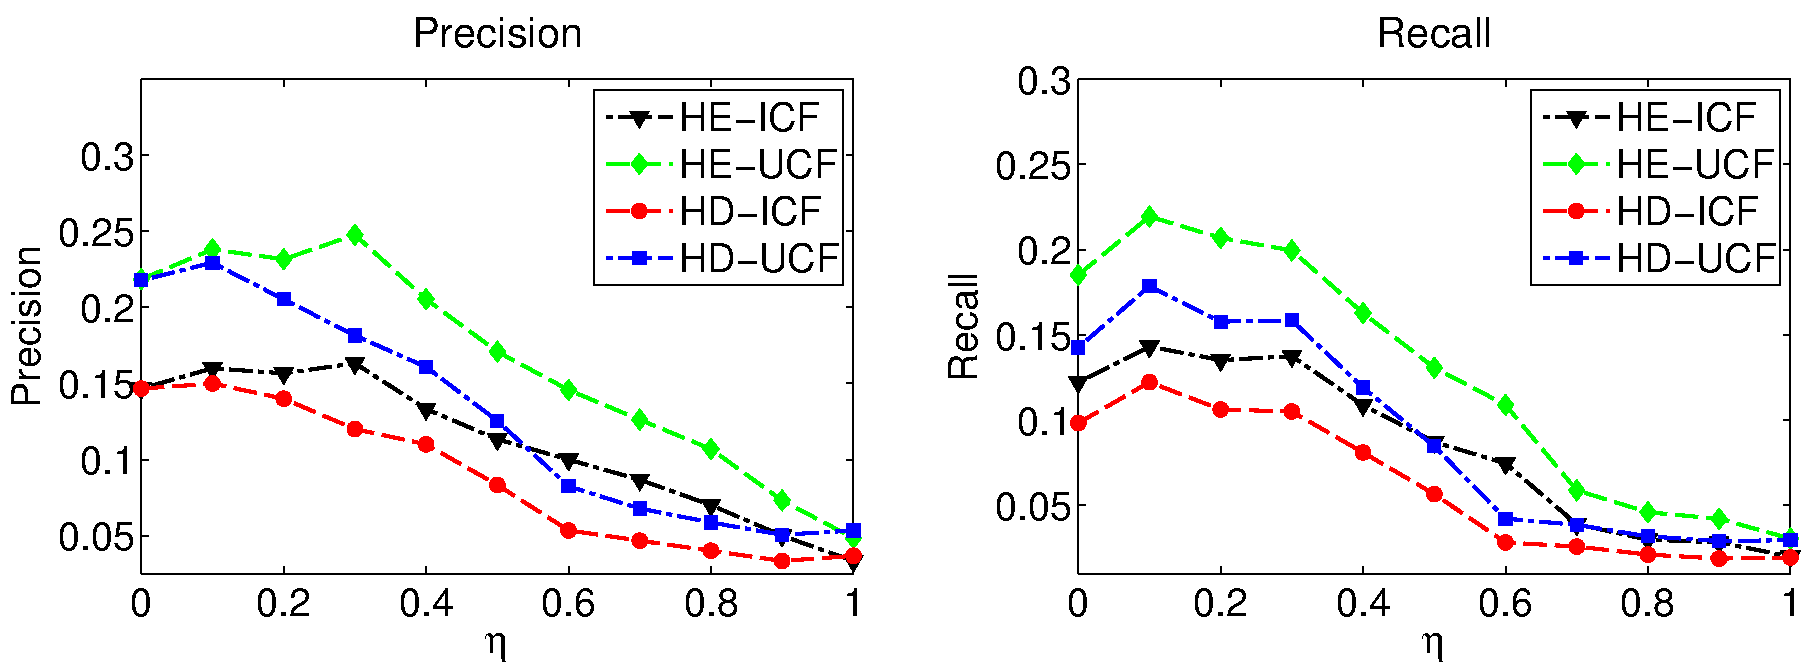
\includegraphics[width=0.95\textwidth]{res/isu_f_pr_weibo_transpose.pdf}\\
  \vspace*{-0.35cm}
  \caption{Comparisons with Different $\eta$}\label{fig:fprweibotrans}
\end{minipage}%%
\begin{minipage}[t]{0.5\linewidth}
\centering
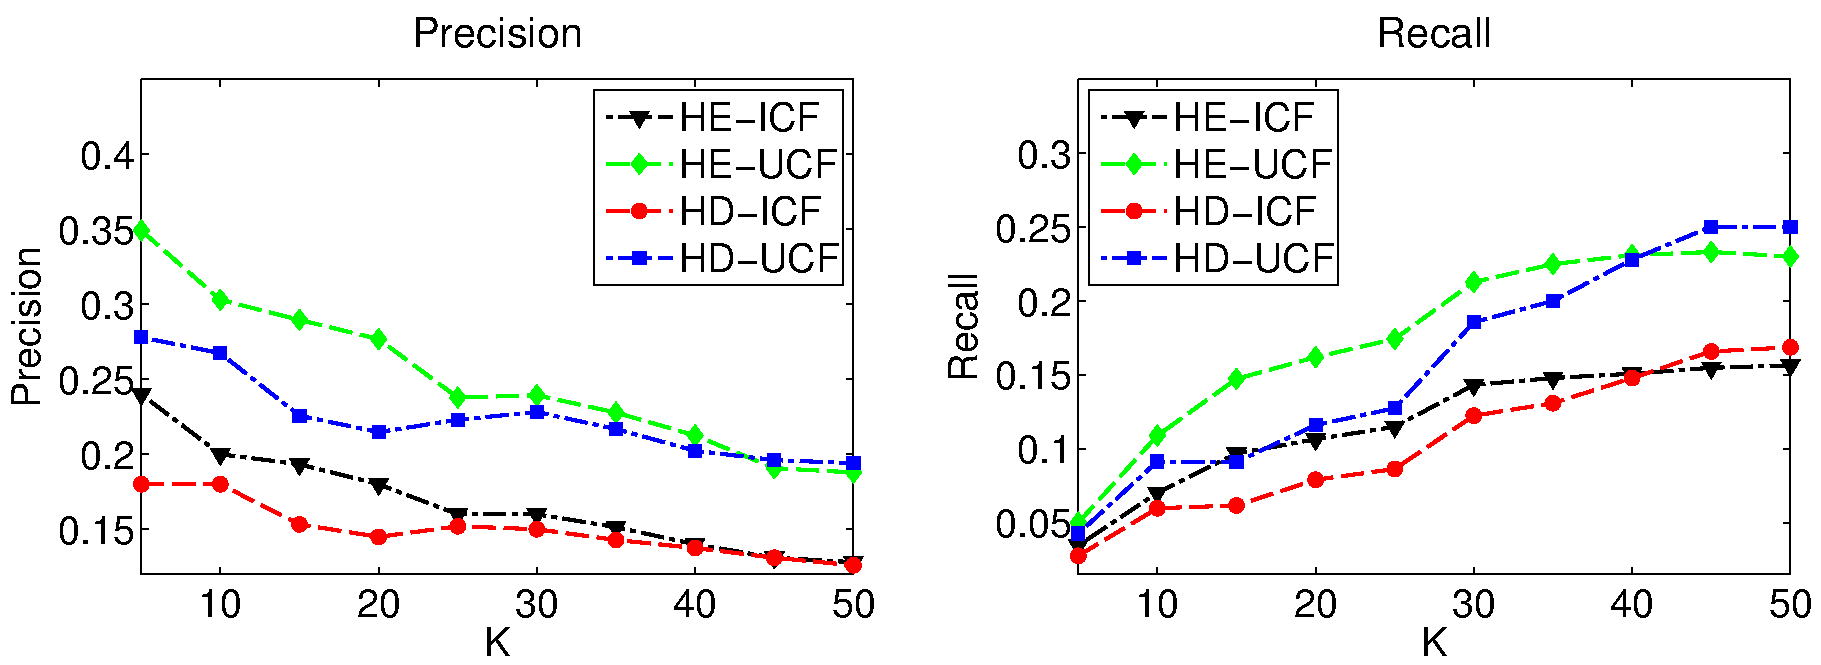
\includegraphics[width=0.95\textwidth]{res/isu_f_pr_weibo.pdf}\\
  \vspace*{-0.35cm}
\caption{Comparisons with Different $|S|$ } \label{fig:fprweibo}
\end{minipage}
\end{figure}


%%%%%%%%%%%%%%%%%%%%%%%%%%%%% Conclusion %%%%%%%%%%%%%%%%%%%%%%%%%%%%%%%%
\vspace*{-0.3cm}
\section{Conclusion}
\vspace*{-0.4cm}
In this paper, we proposed a novel framework to solve the problem of identifying hesitant and interested customers (IHIC) for targeted social marketing.
Specifically, we first proposed an efficient MIP algorithm to calculate the multiple companies' influences on users, and defined two hesitant functions $H(u)$ to measure the user hesitancy. Then we measure the user interest on items
by using two collaborative filtering approaches. Finally, we combined the two types of measures together and proposed the function $P(u,t)$ to identify the hesitant and interested customers. Extensive experiments validated the performance of our proposed approaches. 
%As the first attempt to study the targeted social marketing that taking the influence of multiple companies on users' behaviors into consideration, we hope this study could lead to more future work.

\vspace*{0.2cm}
\noindent
\textbf{Acknowledgement.} This research was partially supported by grants from the National Science Foundation for Distinguished Young Scholars of China (Grant No. 61325010), the Natural Science Foundation of China (Grant No. 61403358), the Fundamental Research Funds for the Central Universities of China (Grant No. WK0110000042) and the Anhui Provincial Natural Science Foundation (Grant No. 1408085QF110). Qi Liu acknowledges the support of the Youth Innovation Promotion Association, CAS.

\vspace*{-0.1cm}

\bibliography{ref}
\bibliographystyle{splncs}

\end{document}
